\documentclass{beamer}
\usepackage{amsmath}
\usepackage{wrapfig}
\usepackage{enumerate}
\usepackage[makeroom]{cancel} % ������������
\usepackage{multicol,multirow} %��������� �������
\usepackage{hyperref}
\usepackage{tabularx}
\usepackage{amsfonts}
\usepackage{amssymb}
\usepackage{amsmath}
\DeclareMathOperator{\Tr}{Tr}
\DeclareMathOperator{\diag}{diag}
\DeclareMathOperator{\conv}{conv}
\DeclareMathOperator{\Rg}{Rank}
\DeclareMathOperator{\Ker}{Ker}
\newcommand{\matrixl}{\left|\left|}
\newcommand{\cbad}{c_{\mathrm{bad}}}
\newcommand{\matrixr}{\right|\right|}
\DeclareMathOperator*{\argmin}{arg\,min}
\newcommand{\h}{\mathbf{h}}
\newcommand{\x}{\mathbf{x}}
\newcommand{\aaa}{\mathbf{a}}
\newcommand{\w}{\mathbf{w}}
\newcommand{\W}{\mathbf{W}}
\newcommand{\y}{\mathbf{y}}
\newcommand{\X}{\mathbf{X}}
\newcommand{\Y}{\mathbf{Y}}
\newcommand{\fx}{\mathbf{f}}
\newcommand{\fs}{\mbox{f}}
\usepackage[cp1251]{inputenc}
\usepackage[russian]{babel}
\usepackage{amsmath,mathrsfs,mathtext}
\usepackage{graphicx, epsfig}
\usetheme{Warsaw}%{Singapore}%{Warsaw}%{Warsaw}%{Darmstadt}
\usecolortheme{sidebartab}
\definecolor{beamer@blendedblue}{RGB}{55,172,32}
%----------------------------------------------------------------------------------------------------------
\title[\hbox to 56mm{Power Flow Feasibility problem  \hfill\insertframenumber\,/\,\inserttotalframenumber}]
{Power flow feasibility problem}
\author[S.E. Volodin]{\large \\Sergei Volodin\\under supervision of Y. Maximov}
\institute{\large Skolkovo Insitute of Science and Technology}

\date{}
%-------------------------------------------------------
\begin{document}
%-------------------------------------------------------
\begin{frame}
%\thispagestyle{empty}
\titlepage
\end{frame}
%-------------------------------------------------------
\begin{frame}{The problem}
\begin{enumerate}
\item Large-scale power grids
\item Need to know if a regime of the grid is <<normal>>, <<safe>>
\item Ohm's law $\Rightarrow$ quadratic equations:
$$y_i=f_i(x)=x^TA_ix+2b_i^Tx$$
$y$ (regime) known, $x$ is not
\item Need to determine if $\exists x\colon y=f(x)$ (means <<safe>>)
\end{enumerate}

This problem is known as Power Flow Feasibility problem.

To solve it, the image $f(\mathbb{R}^n)$ must be examined
\end{frame}

\begin{frame}{The solution}
Given: the map $f\colon\mathbb{R}^n\to\mathbb{R}^m$, $f_i(x)=x^TA_ix+2b_i^Tx,\,A_i^T=A_i$
Proposed algorithm for examining $F=f(\mathbb{R}^n)$:
\begin{itemize}
\item {\bf Input:} $y^0\in F$, direction $c_+\colon c_+\cdot A>0$
\item {\bf Output:} value $z_{\max}$ s.t. the cut $Q(c_+,z_{\max}, F)$ is convex
\end{itemize}
Solution overview:
\begin{enumerate}
	\item Discovering boundary nonconvexities $\{F_i\}$ close to $y^0$
	\item Projecting to $c_+$: $(F_i,c_+)$
	\item Calculating $z_{\max}=\inf\limits_i \inf\limits_{y\in F_i}(c_+,y)$
\end{enumerate}
$Q(c_+,z,F)=\{y\big| (y-y^*,c_+)\in[0,z]\}\cap F$, $y^*$~--- touching point of hyperplane $c_+$\\
\centering 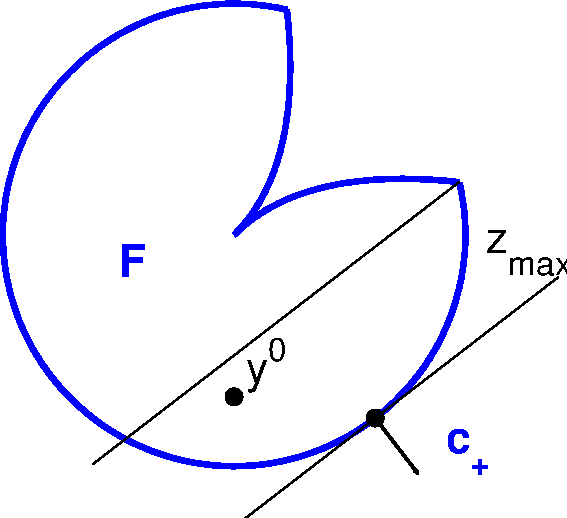
\includegraphics[width=80px]{cut}

\end{frame}

\begin{frame}{The solution}
Solution in details:
\begin{enumerate}
\item Rewrite $z_{\max}=\inf\limits_{c_{\cbad}}z(c)$~--- constrained optimization task
\item Using the Gradient projection method
\item Special technique for projection using geometry of $\cbad$
\end{enumerate}
\centering 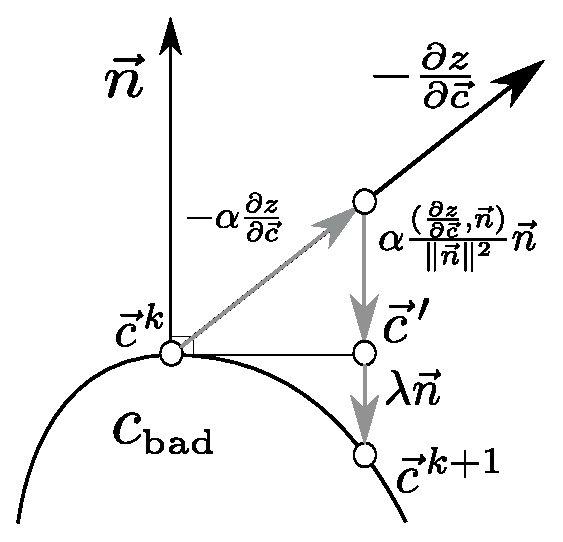
\includegraphics[width=150px]{c_bad_continuum}
\end{frame}

\begin{frame}{Numerical experiment}
An example: $f\colon \mathbb{R}^4\to\mathbb{R}^4$
\begin{itemize}
\item 4 local minima
\item Global minimum found
\end{itemize}
\centering 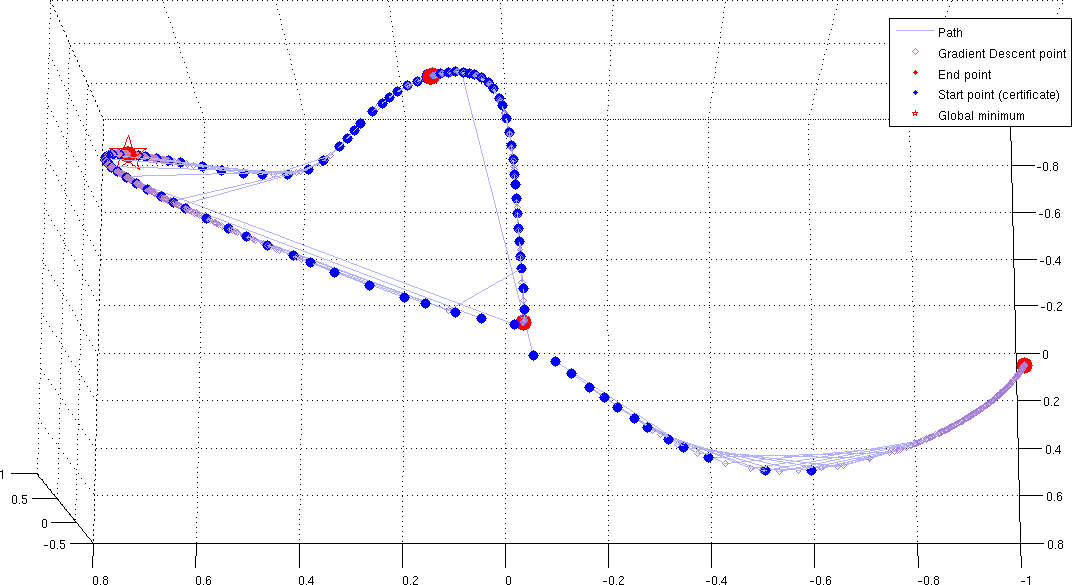
\includegraphics[width=300px]{example03_cbad_91pts_03.png}
\end{frame}

\begin{frame}{Results}
Algorithm for examining the set of <<safe>> regimes was proposed:
\begin{enumerate}
\item Can determine if the whole subset is <<safe>> at one run
\item Cuts convex parts of the image $F$
\item General case when the set of nonconvexities is a continuum was considered
\item Algorithm was tested on a number of maps $f$
\end{enumerate}
Plan:
\begin{enumerate}
	\item $\mathbb{C}$ case
	\item Testing for higher dimensions
\end{enumerate}
%\vspace{40px}
\begin{tabular}{cccc}
\begin{minipage}{0.23\textwidth} 
\hspace*{-30px}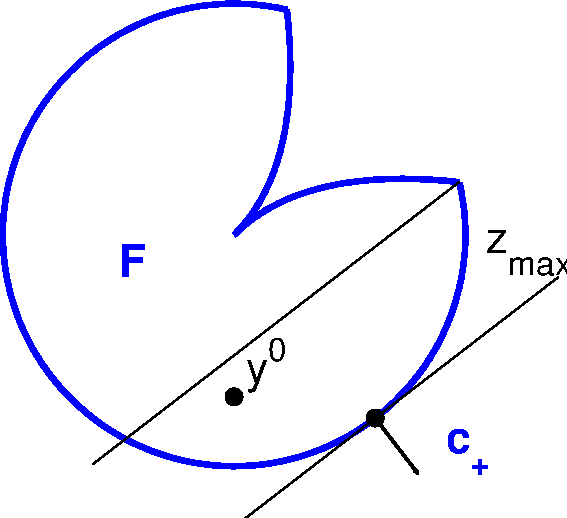
\includegraphics[height=60px]{cut}
\end{minipage} &
\begin{minipage}{0.23\textwidth}
\hspace*{-40px}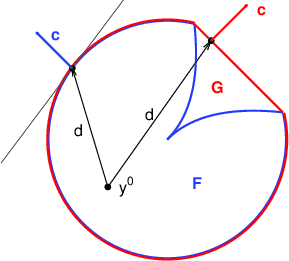
\includegraphics[height=60px]{alg_idea20}
\end{minipage} &
\begin{minipage}{0.23\textwidth}
\hspace*{-35px}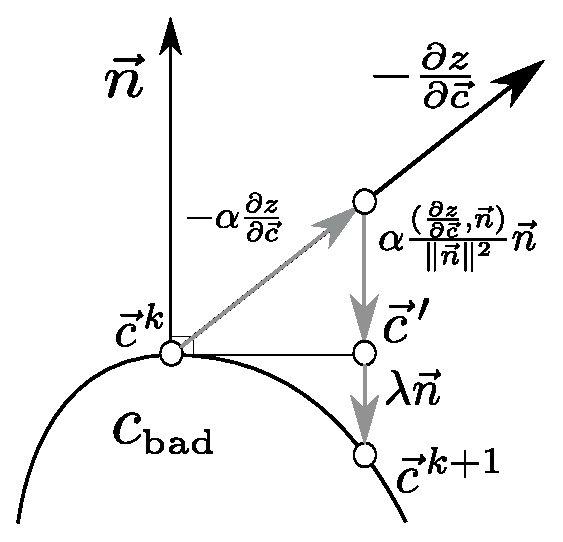
\includegraphics[height=60px]{c_bad_continuum}
\end{minipage} &
\begin{minipage}{0.31\textwidth}
\hspace*{-35px}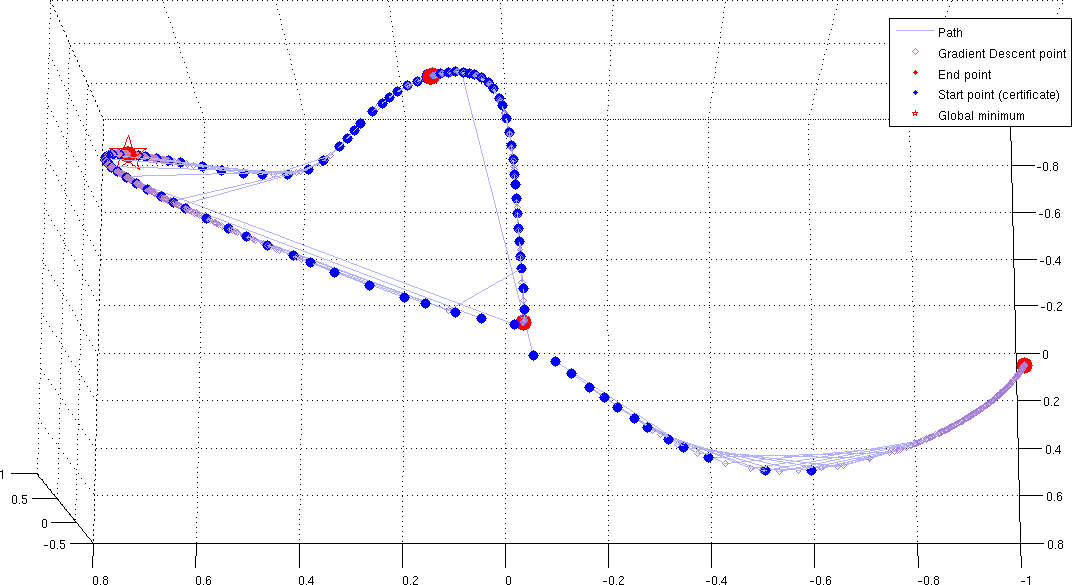
\includegraphics[height=60px]{example03_cbad_91pts_03.png}
\end{minipage}
\end{tabular}
\end{frame}
\end{document} 